\chapter{Prototype System Design}
\label{chp:sys_design}

\noindent In this chapter, it will cover system design progress of the prototype system along with explanation and analysis. The prototype system is designed based on preliminary studies from previous chapter. There will be different implementation solutions to the prototype working scenario  discussed and evaluated in this chapter. After evaluating these solutions, it will come up with the fit solution to the prototype working scenario. 

\section{Prototype System Network}

\noindent In the original \gls{webrtc} application implementation, it uses mesh network because \gls{webrtc} means to be the peer to peer communication method bypass the third party server. However, the prototype system will use centralized server network to control and route the communication channels between different types end points. In this section, it will describe the reason to use centralized server network rather than mesh network.

\subsection{Mesh Network}

\par A mesh network is a network topology in which each node (called a mesh node) relays data for the network, the illustration of the network is shown in Figure \ref{fig:mesh_network}. All nodes cooperate in the distribution of data in the network. When \gls{webrtc} designed, it considered as mesh network using and take the advantages of the mesh network. Mesh network provides point-to-point line configuration makes identification and isolation of faults easy. The messages travel through a dedicated line in the mesh network, directly to the intended recipient. More privacy and security are thus enhanced. If a fault occurs in a given link of the network, only those communications between that specific pair of devices sharing the link will be affected.\cite{wiki:mesh_network}

\par However, with the design of mesh network, the more extensive the network, in terms of scope or of physical area, the greater the investment necessary to build it will be, due, among other considerations, to the amount of cabling and the number of hardware ports it will require.
Every device must be connected to every other device, installation and re-connection are difficult. The huge bulk of the wiring can often be greater than the available space in the ceiling or under floors can accommodate.

\begin{figure}
	\centering
    	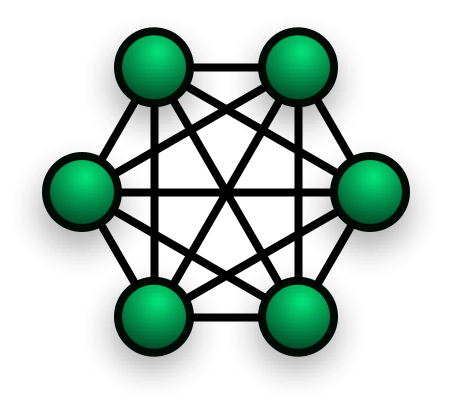
\includegraphics[width=0.40\textwidth,natwidth=610,natheight=642]{figs/mesh_network.png}
  	\caption{Illustration of a Mesh Network \cite{wiki:mesh_network}}
  	\label{fig:mesh_network}
\end{figure}

\par Considering the prototype system case, a real-time communication system, the scaling problem in the feature will eventually be the top priority issue. With the mesh network, it is difficult and impossible to scale the system with the control since the network scales by the unknown end points.There is a similar production application called \textit{appear.in}. It is a video conversations application with up to 8 people in the browser. \textit{appear.in} uses peer-to-peer communication, meaning that the video streams are sent directly between the browser clients. Nothing is stored on the server and all the communication is encrypted over SSL. But the limit of 8 clients in one conversation is mainly because the client browser it self can not handle too many peer connections. Because according to mesh network, every client in the conversation would set up one unique \gls{webrtc} \textit{RTCPeerConnection} object and one unique media stream exchange channel on the client, it consumes client computer resources a lot. Thus, the prototype system will not use mesh network as the system network architecture in order to avoid the future scaling problem. The advantages of the mesh network is well implemented in the \gls{webrtc} api, then the prototype system will keep these advantages to keep the point-to-point lines isolated with each other and keep the point-to-point communication more private and secure.

\subsection{Centralized Network}

\par Centralized network is a type of network where all users connect to a central server, which is the acting agent for all communications. This server would store both the communications and the user account information. Most public instant messaging platforms use a centralized network. It is also called as centralized server-structure.\cite{webopedia:centralized_network} It is similar network architecture shown in Figure \ref{fig:system_network}.

\begin{figure}
	\centering
    	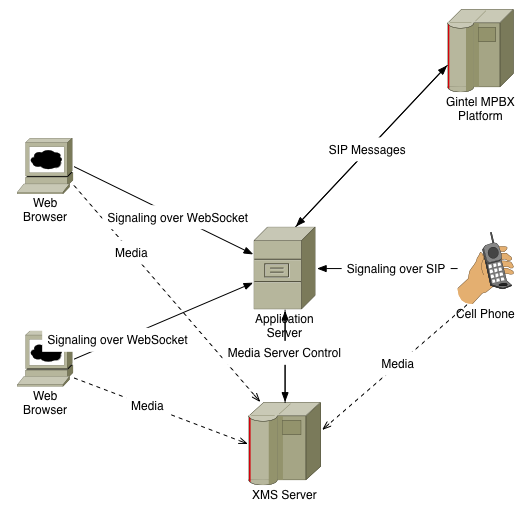
\includegraphics[width=0.70\textwidth,natwidth=610,natheight=642]{figs/system_network.png}
  	\caption{Prototype System Network}
  	\label{fig:system_network}
\end{figure}

\par The advantages of centralized server network are centralized control of the system, centralized observation of the system and light requirement for the client . In the prototype system, there are application server and media server to handle the application logic business and media stream exchange business(see in Figure \ref{fig:system_network}). Although every clients communicate with application to do the \gls{webrtc} signaling, the media stream is not go through the application server, it goes through the media server only. Furthermore, every client creates single \gls{webrtc} connection pair with the one resource on XMS media server, the advantage of point-to-point line configuration is still kept in the system. As client aspect, it still makes peer-to-peer media stream connection based on \gls{ssl}. The function of XMS media server is to combine more than two of the peer resources into one conference resource in order to set up the multimedia conference channel. More detail about XMS media server handling will be covered in Chapter \ref{chp:sys_imp}.

\par The other important advantage of centralized server network is that the application server and media server can observe the condition and quality of the real-time conversation to administrate the routing and quality improvement process. For this reason, the media stream quality on every end point will be more stable and better quality control. Since the prototype application is to integrate with traditional telephony network, it is important to provide similar quality control and fault tolerant mechanism in the prototype system.

\par Regarding to centralized server network, it is possible to use different signaling protocol on \gls{webrtc} browser clients to application server and \gls{sip} clients to application server. The benefits to have different signaling protocols in prototype system is to keep the \gls{webrtc} clients and the \gls{sip} clients in their own traditional working process, there will be no compatibility for both sides. Moreover, it will be easier for different existing \gls{webrtc} commercial services and \gls{sip} commercial services to integrate with the prototype system in order to communicate with each other network.

\par The disadvantage of centralized server network would be the application server and media server itself as well. During the development of the prototype system, it is easy to figure out that the machine to host the application server and media server is not powerful enough to handle too much client connection and media stream connection. When it meets the scaling issue, the application server and media server need to be distributed in multiple server host and consume powerful server machines. The cost of the entire system is higher than the mesh network solution.

\par As a conclusion of these two types network architecture, for this prototype system, it will be centralized server network, Figure \ref{fig:system_network}, to be implemented because it is more suit to the goal of this thesis to be integrated with traditional telephony network usage.

\section{Prototype Implementation Framework}

\noindent Since \gls{webrtc} is a web \gls{api}, the prototype application will be a web application. There are many different web application framework nowadays to provide rich-client web application. In this section, some of the web application framework will be discussed to figure out which framework is best solution to the prototype scenario. Furthermore, application server will be discussed with different implementation solutions since it does signaling and bridge the \gls{sip} network and clients.

\subsection{Client Implementation Framework}

\noindent To choose web application framework to implement the client application in this thesis scenario, the main fact is that if the web  application framework is fit to the real time communication application and if the framework has the ability to integrate with \gls{webrtc} \gls{api}. After research about these kinds of web application framework, it narrows down to three main framework to discuss.

\textbf{AngularDart :}

\par AngularDart is a framework for building web-apps in Dart. Dart is an open-source Web programming language developed by Google. It is a class-based, single inheritance, object-oriented language with C-style syntax. It supports interfaces, abstract classes, reified generics, and optional typing. Static type annotations do not affect the runtime semantics of the code. Instead, the type annotations can provide documentation for tools like static checkers and dynamic run time checks.\cite{wiki:dart} Because most of the script language is not type strict, it is easy to mess up the code and value type in script language. Moreover, Dart has Dart-to-JavaScript compiler,dart2js, it makes Dart can be used in client and server both. Addition to AngularJs framework in Dart, it provide a professional web application structure to the developer to implement. More about AngularJs notable features will be covered in the later AngularJs solutions. 

\par The \gls{webrtc} implementation in Dart is in this repository: \url{https://github.com/br1anchen/AngularDart_webRTC}. The Code Snippet \ref{code:dart_webrtcctrl} shows the main controller in AngularDart. The line 5 is to import \gls{webrtc} client class \textit{speack\_client.dart}, the class has all the \gls{webrtc} \gls{api}s implemented in Dart. Line 23 is to initialize the \textit{SpeakerClient} object and set the arguments WebSocket url and room name. They are used for signaling in WebSocket Protocol.

\par However, after implementation of client application and server back-end in Dart. There is a critical bug in the current Dartium browser. The Dart SDK ships with a version of the Chromium web browser modified to include a Dart \gls{vm}. Dartium browser can run Dart code directly without compilation to JavaScript. It is intended as a development tool for Dart applications, rather than as a general purpose web browser. When embedding Dart code into web apps, the current recommended procedure is to load a bootstrap JavaScript file, "dart.js", which will detect the presence or absence of the Dart \gls{vm} and load the corresponding Dart or compiled JavaScript code, respectively, therefore guaranteeing browser compatibility with or without the custom Dart VM.\cite{wiki:dart} 
\par The issue noticed as \textbf{RtcPeerConnection.addIceCandidate results in a NotSupportedError: Internal Dartium Exception} in the Dart Google Project issues.\cite{bug:dartium} The sample code in the \gls{webrtc} Dart implementation shown in Code Snippet \ref{code:dart_add_ice}, line 1 is to create \textit{RTCPeerConnection} object. From line 5 to line 13 is to send message to server when \textit{RTCPeerConnection} object get \textit{onIceCandidate} event witch \gls{ice} candidate information. Line 17 is to bind the message listener event to Dart function \textit{onCandidate.listen}. From line 21 to line 30 is the Dart function to create \textit{RTCIceCandidate} object and add to \textit{RTCPeerConnection} object. The bug issue happens on line 27, when the \textit{RTCPeerConnection} call \textit{addIceCandidate} function, it is not allowed to have callback function in current version Dartium.

\begin{lstlisting}[caption={Add IceCandidate in Dart},label={code:dart_add_ice}]
var pc = new RtcPeerConnection(_iceServers, _dataConfig);

....

    pc.onIceCandidate.listen((e){
      if (e.candidate != null) {
        _send('candidate', {
          'label': e.candidate.sdpMLineIndex,
          'id': id,
          'candidate': e.candidate.candidate
        });
      }
    });
    
...

get onCandidate => _messages.where((m) => m['type'] == 'candidate');

...

onCandidate.listen((message) {
	var candidate = new RtcIceCandidate({
		'sdpMLineIndex': message['label'],
        'candidate': message['candidate']
    });

    _connections[message['id']].addIceCandidate(candidate,(){},(e){
    		print('add ice candidate error');
    });
});

...
\end{lstlisting}

\par There is a work around solution in one Stack Overflow\footnote{Stack Overflow is a privately held website, the flagship site of the Stack Exchange Network, created in 2008 by Jeff Atwood and Joel Spolsky, as a more open alternative to earlier Q\&A sites such as Experts Exchange.} answer: \url{http://stackoverflow.com/questions/20404312/how-to-call-addicecandidate-in-dart}. The fix method is to use \textit{js-interop} library to use pure JavaScript code in Dart to call the \gls{webrtc} Web \gls{api} instead of Dart \gls{webrtc} interface.
\par Mozilla's Brendan Eich, who developed the JavaScript language, stated that:

\textit{"I guarantee you that Apple and Microsoft (and Opera and Mozilla, but the first two are enough) will never embed the Dart VM. So 'Works best in Chrome' and even 'Works only in Chrome' are new norms promulgated intentionally by Google. We see more of this fragmentation every day. As a user of Chrome and Firefox (and Safari), I find it painful to experience, never mind the political bad taste."}\cite{wiki:dart}

\par Since Dart in not support to most modern web browser like FireFox, will not be used in this prototype.

\textbf{Sipml5 + webrtc2sip:}

\begin{figure}
	\centering
    	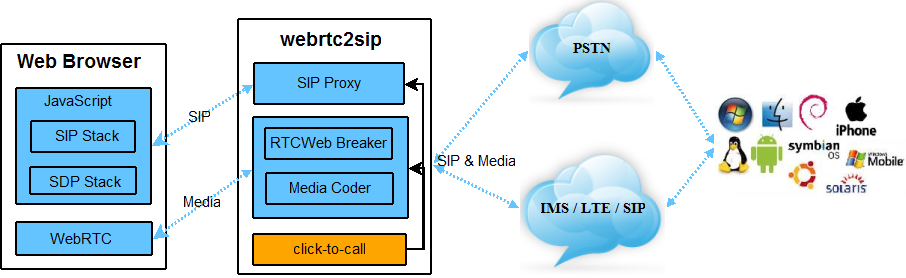
\includegraphics[width=0.80\textwidth,natwidth=610,natheight=642]{figs/sipml5_network.png}
  	\caption{Sipml5 and webrtc2sip Network}
  	\label{fig:sipml5_network}
\end{figure}

\par Sipml5 is the world's first open source \gls{html5} \gls{sip} client entirely written in JavaScript for integration in social networks (FaceBook, Twitter, Google+), online games, e-commerce websites, email signatures. The media stack rely on \gls{webrtc}. The client can be used to connect to any \gls{sip} or \gls{ims} network from your preferred browser to make and receive audio/video calls and instant messages.\cite{website:sipml5}

\par Sipml5 provides whole client solution to communicate with other kind of signaling real-time communication network. The \gls{sip} and \gls{sdp} stacks are entirely written in JavaScript and the network transport uses WebSockets as per draft-ibc-sipcore-sip-websocket. However the community of sipml5 is not so active, the issues and source code on sipml5 source code project website \url{https://code.google.com/p/sipml5/} are not updated regularly. Like the Figure \ref{fig:sipml5_network} showing, it works with media gateway webrtc2sip.

\par webrtc2sip is a smart and powerful gateway using \gls{webrtc} and \gls{sip} to turn your browser into a phone with audio, video and \gls{sms} capabilities. The gateway allows your web browser to make and receive calls from/to any \gls{sip}-legacy network or \gls{pstn}.
The gateway contains four modules: \gls{sip} Proxy, RTCWeb Breaker, Media Coder, Click-to-Call.\cite{website:webrtc2sip}

\par In the prototype working scenario, it is necessary to have media gateway to communicate with \gls{sip}-legacy network. Since the current \gls{pstn} using in this prototype go through Gintel \gls{mpbx} Platform, it is necessary to use RTCWeb Breaker to be able to connect the browser to a SIP-legacy endpoint.

\par Therefore, the test for Sipml5 and webrtc2sip solution is based on the live demo \url{http://sipml5.org/call.htm}. But even with the RTCWeb Breaker, the test is still failed to call any number through the target \gls{pstn}. Since most of the source code of these two framework are hidden from the encapsulation, it is impossible to debug which part of the testing system is the problem. In the test, the registration for \gls{sip} client is successful, but there are 'too long message' in the \gls{sip} error message got from the \gls{sip} server. It means that the sipml5 and webrtc2sip network architecture is not compatible with the target \gls{pstn} through the Gintel \gls{mpbx} Platform. This solution can not be used in the prototype system.

\textbf{AngularJs + Socket.IO:}

\par AngularJS is built around the belief that declarative programming should be used for building user interfaces and wiring software components, while imperative programming is excellent for expressing business logic. The framework adapts and extends traditional \gls{html} to better serve dynamic content through two-way data-binding that allows for the automatic synchronization of models and views. As a result, AngularJS de-emphasizes \gls{dom} manipulation and improves testability. Angular follows the \gls{mvc} pattern of software engineering and encourages loose coupling between presentation, data, and logic components. Using dependency injection, Angular brings traditional server-side services, such as view-dependent controllers, to client-side web applications. Consequently, much of the burden on the backend is reduced, leading to much lighter web applications.\cite{wiki:angularjs}

\par AngularJs is perfect for single-page web application, the framework features provide developer a professional way to structure the web application in JavaScript. Moreover, the developer community of AngularJs is quite active, there are a lot of different Angular module services to provide the different interfaces against different web \gls{api}s.In the prototype, there will be several third party Angular module library to be used in order to integrate with some advanced JavaScript library or web \gls{api}s in Angular style.

\par Socket.IO is a JavaScript library for realtime web applications. It has two parts: a client-side library that runs in the browser, and a server-side library for node.js. Both components have a nearly identical \gls{api}. Socket.IO primarily uses the WebSocket protocol, but if needed can fallback on multiple other methods, such as Adobe Flash sockets, \gls{jsonp} polling, and \gls{ajax} long polling, while providing the same interface. Although it can be used as simply a wrapper for WebSocket, it provides many more features, including broadcasting to multiple sockets, storing data associated with each client, and asynchronous I/O.\cite{wiki:socketio} In the prototype application, Socket.IO is used in WebSocket protocol because the WebSocket protocol provides full-duplex communications channels over a single \gls{tcp} connection. Then the communication channel will be active and real time between the clients and server during the whole connecting procedure. It fits the real time communication application requirement.

\par After test demo client application implemented in AngularJs and Socket.IO frameworks, it works fine with the basic \gls{webrtc} functions and simple \gls{sip} registration against \gls{sip} server to target \gls{pstn}. The final decision of the client implementation framework of prototype system will be AngularJs and Socket.IO.

\subsection{Server Implementation Framework}

\noindent Since the client side will use Socket.IO as communication protocol library, the server back-end in the prototype system will use Node.js as server implementation framework. In thist section, more detail about comparison and differences of Node.js against traditional web service back-end (in Java, ASP .NET\footnote{ASP.NET is a server-side Web application framework designed for Web development to produce dynamic Web pages. It was developed by Microsoft to allow programmers to build dynamic web sites, web applications and web services.\cite{wiki:asp}} or \gls{php}) will be covered.

\textbf{Node.js:}

\par Node.js is a software platform for scalable server-side and networking applications. Node.js applications are written in JavaScript, and can be run within the Node.js runtime on Mac OS X, Windows and Linux with no changes. Node.js applications are designed to maximize throughput and efficiency, using non-blocking I/O(Input/Output) and asynchronous events. Node.js applications run single-threaded, although Node.js uses multiple threads for file and network events. Node.js is commonly used for real time applications due to its asynchronous nature.\cite{wiki:nodejs}

\par At high levels of concurrency server needs to go to asynchronous non-blocking, otherwise there will be blocking \gls{io} on the server to delay other \gls{io} process. The issue is that if any part of the server code blocks, on the traditional server framework,  it is going to need a thread. And at these levels of concurrency, it can’t keep creating threads for every connection. Then the whole codepath needs to be non-blocking and synchronized, not just the \gls{io} layer. This is where Node excels, shown in Figure \ref{fig:nodejs}. The main difference between Figure \ref{fig:nodejs} and Figure \ref{fig:threading_java} is the way of server to handle the requests. On Node.js server, it handles all the requests in asynchronous threads after the requests are delegated from event loop. But on multiple threaded server, programming language used on these server mostly does not support for the async pattern. Then it would not matter whether raw \gls{nio} performance is better than Node or any other benchmark result.

\begin{figure}
	\centering
    	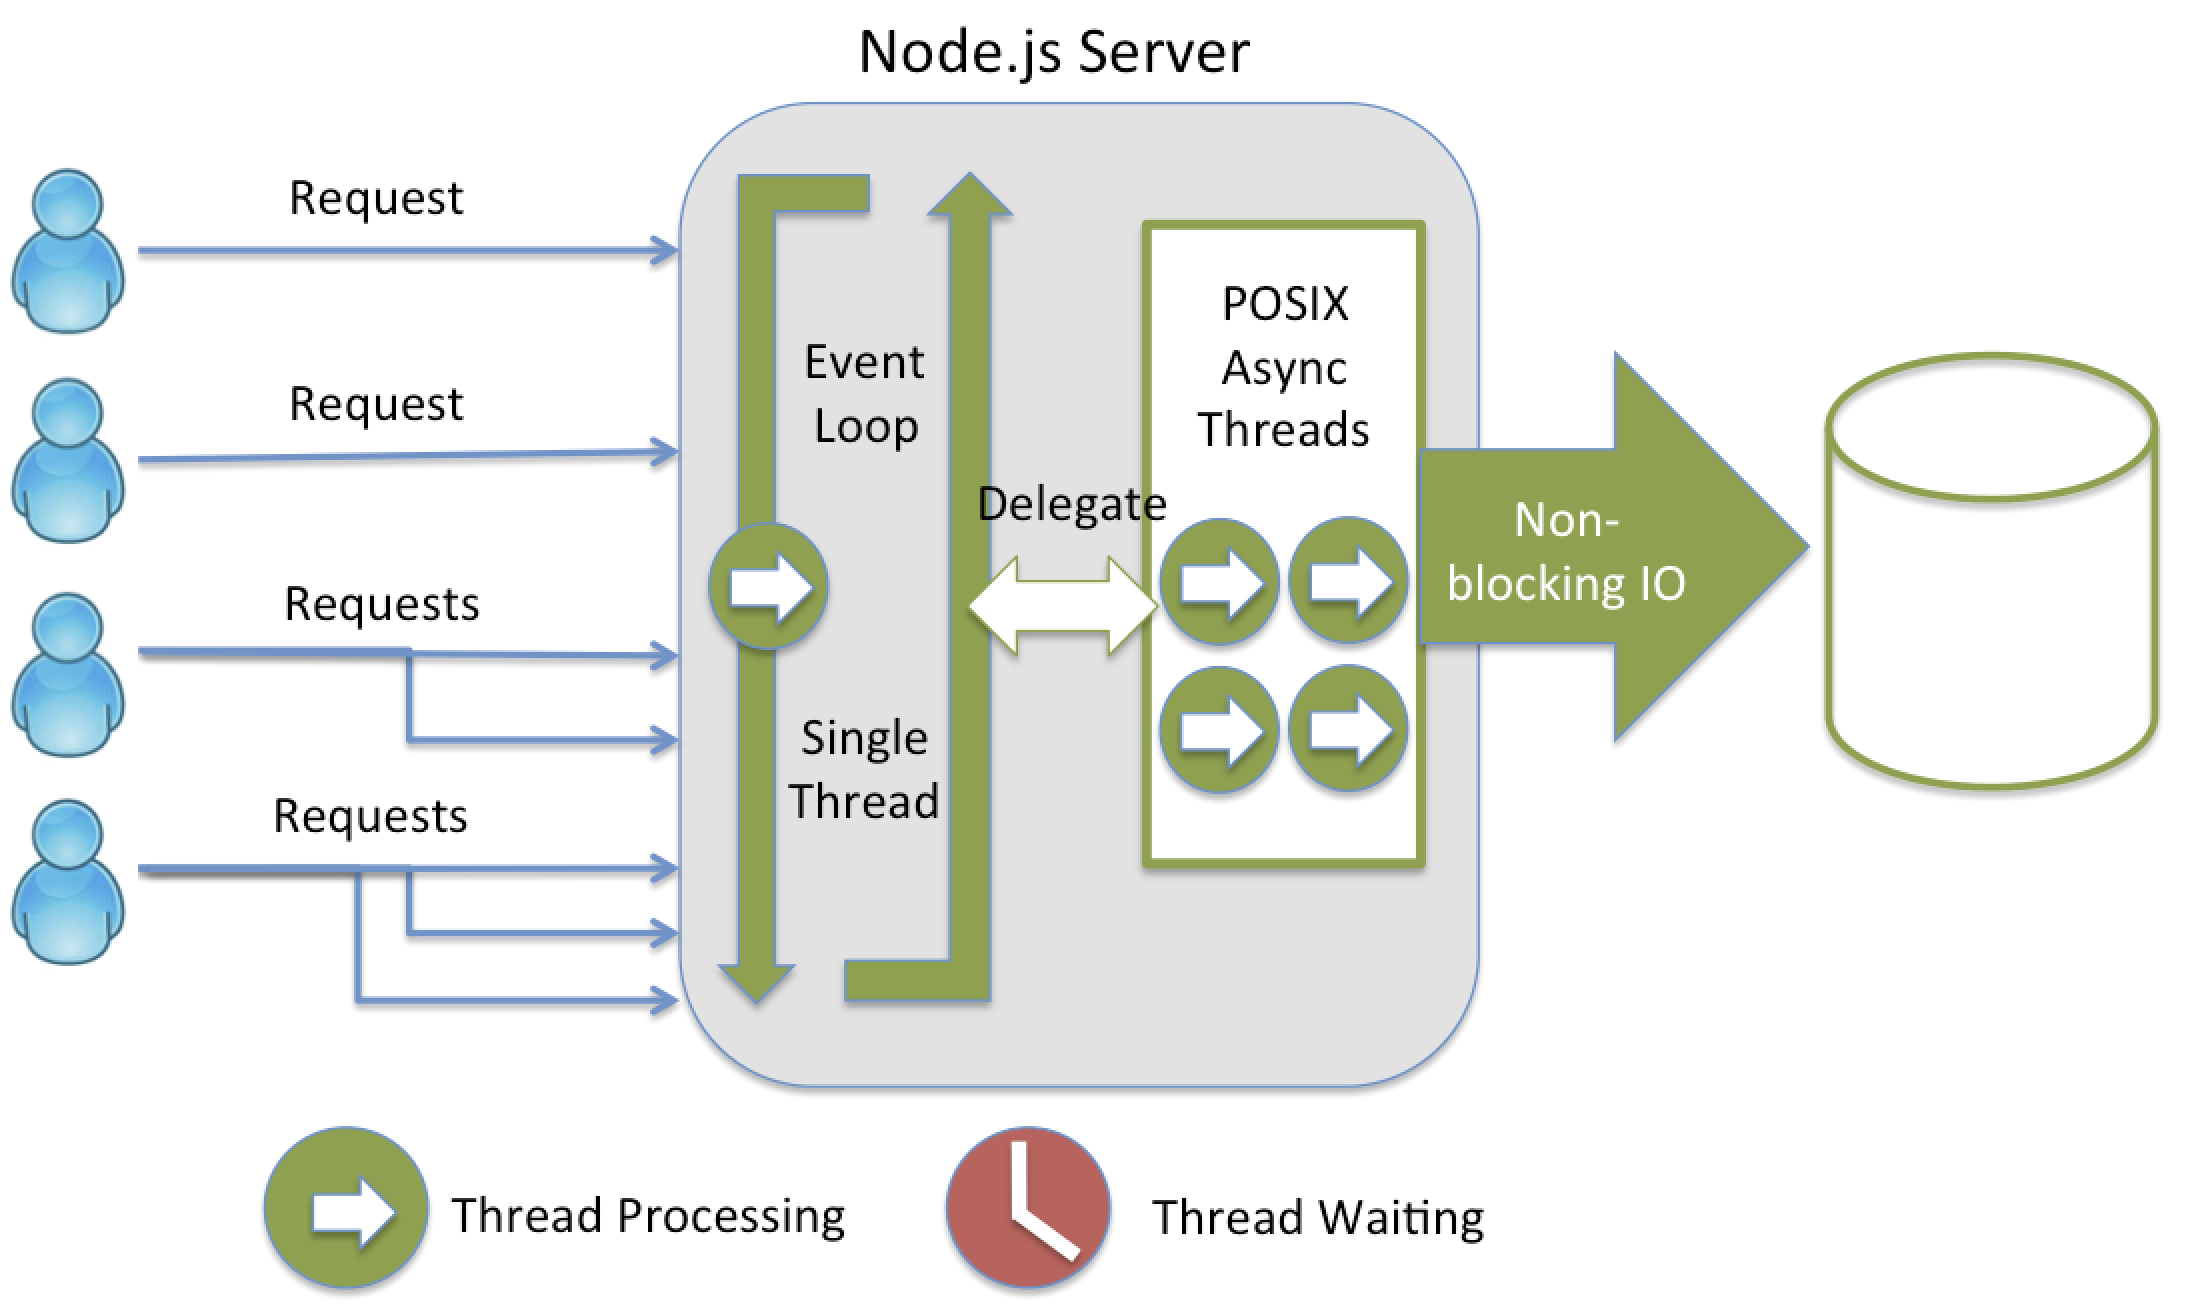
\includegraphics[width=0.60\textwidth,natwidth=610,natheight=642]{figs/nodejs.png}
  	\caption{Node.js Non-blocking I/O\cite{strongloop:nodejs}}
  	\label{fig:nodejs}
\end{figure}

\begin{figure}
	\centering
    	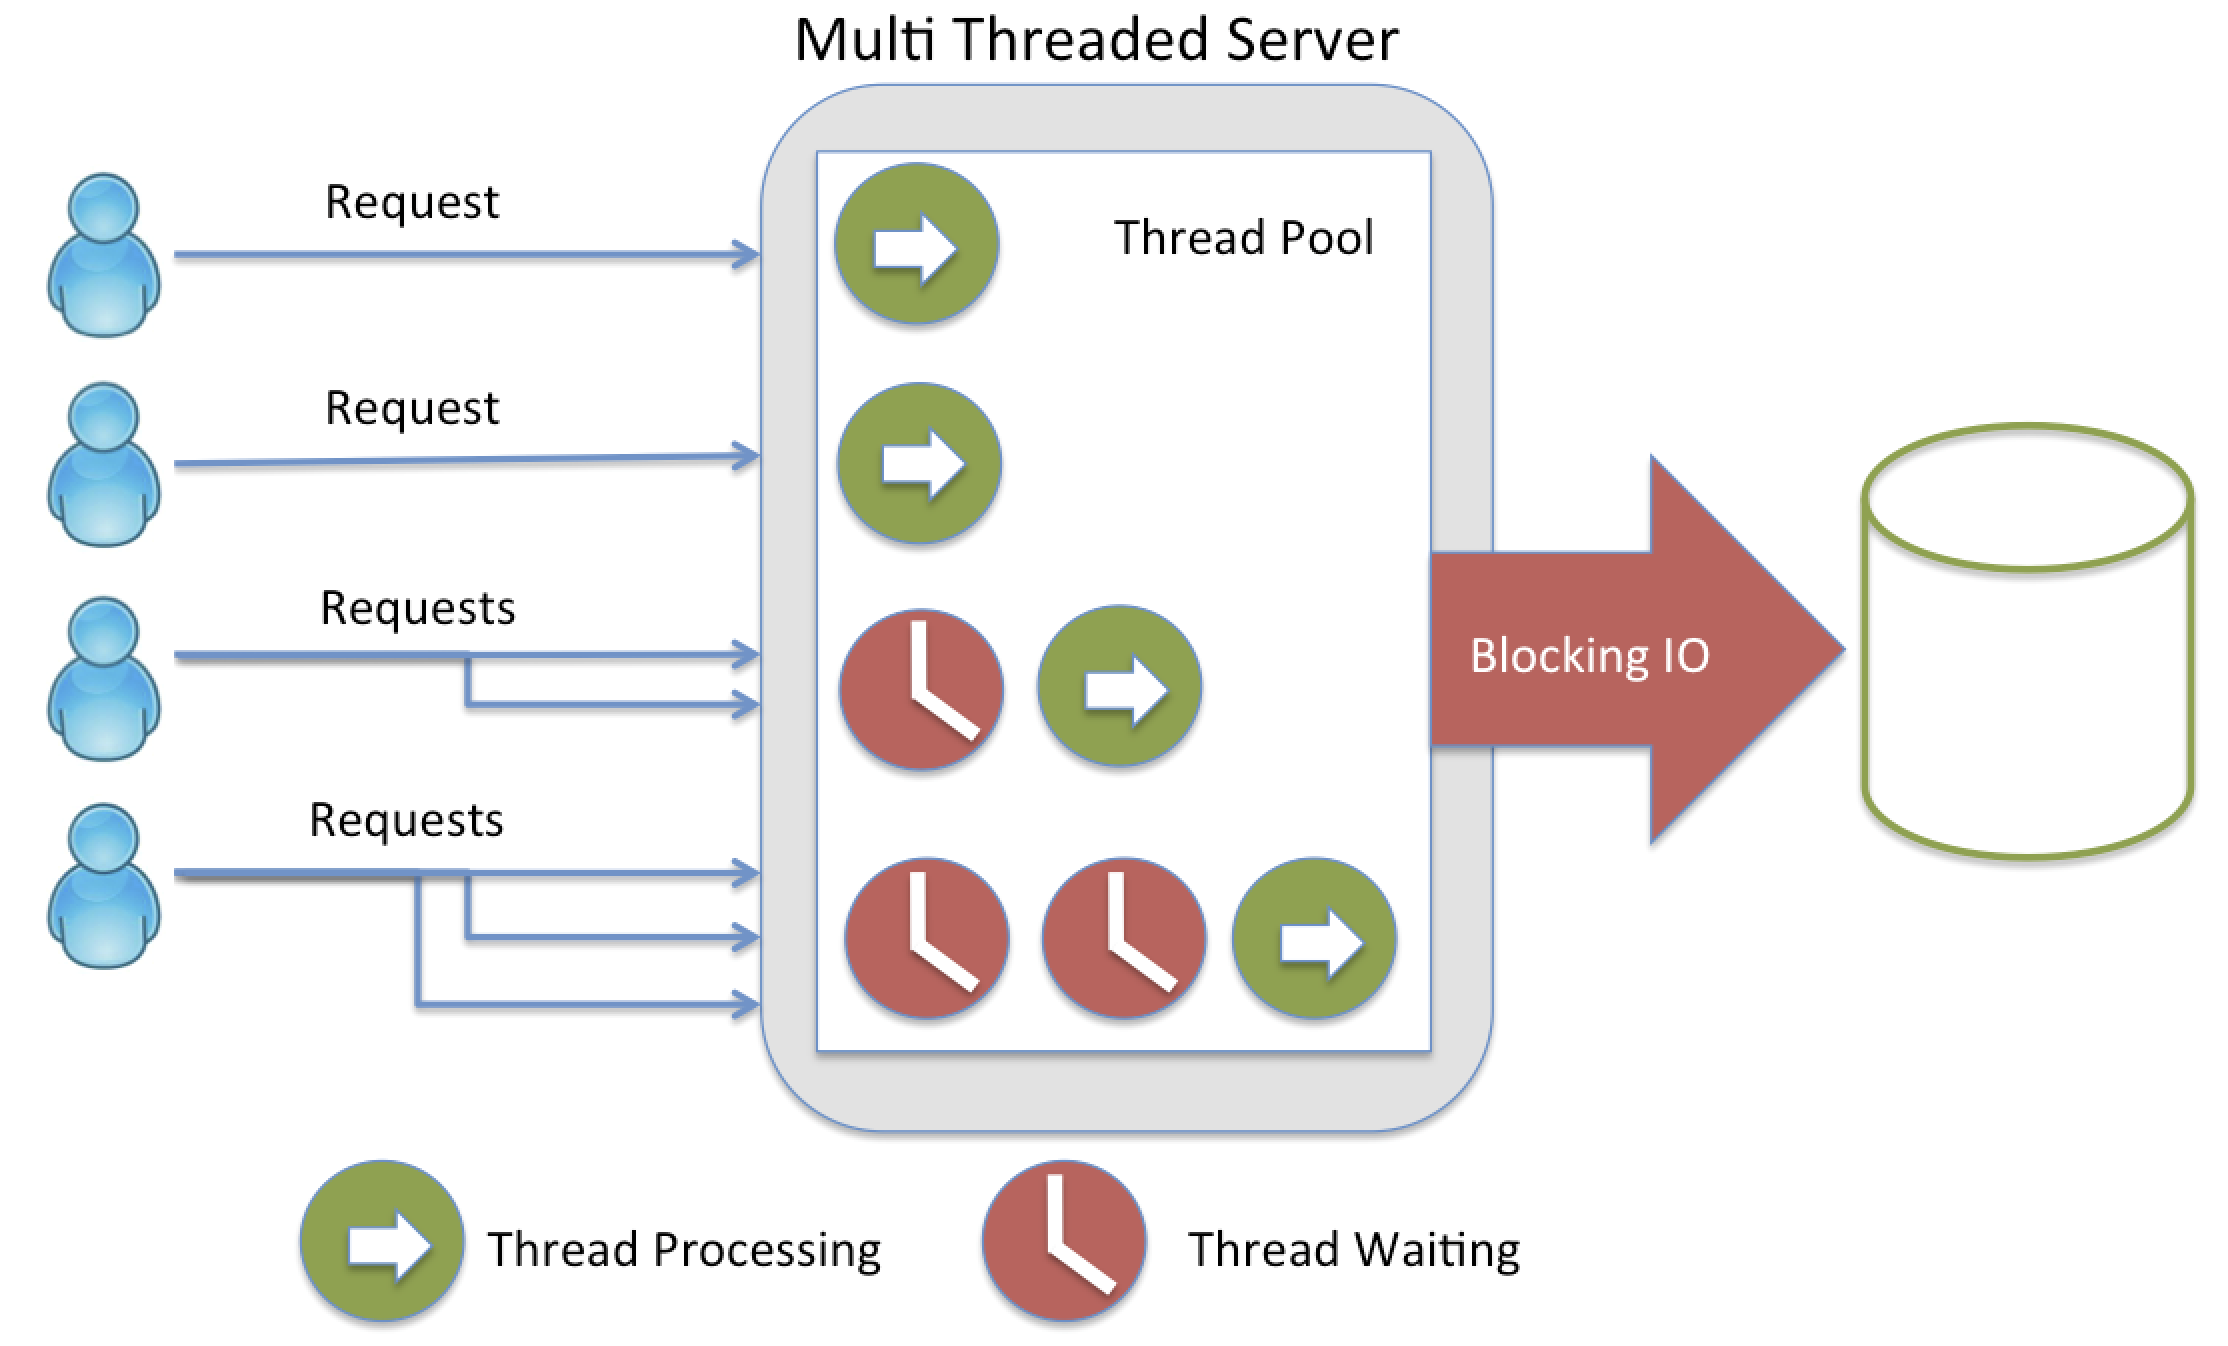
\includegraphics[width=0.60\textwidth,natwidth=610,natheight=642]{figs/threading_java.png}
  	\caption{Multiple Threaded Server\cite{strongloop:nodejs}}
  	\label{fig:threading_java}
\end{figure}

\par Since the prototype is a real-time communication application, it is better to use Node.js as back-end server rather than multiple threaded server. Moreover, the WebSocket protocol framework used on client side has good server side solution based on Node.js, it makes the development of the prototype system much easier to implement. The prototype system is a centralized server network, the communication between application server to XMS server will be hold on normal \gls{http}/\gls{https} protocol, Node.js provides these protocol communication as well, no need to host any additional web server software such as Apache\footnote{The Apache HTTP Server, commonly referred to as Apache, is a web server application notable for playing a key role in the initial growth of the World Wide Web.\cite{wiki:apache}}.

\par For the other part of the prototype, \gls{sip} network, there is a existing Node.js module can be used as \gls{sip} stack on Node.js server. sip.js is a \gls{sip} stack for node.js. It implements tranaction and transport layers as described in RFC3261\footnote{SIP: Session Initiation Protocol}.\cite{github:sipjs} Although sip.js is not production framework yet, it is one of the few \gls{sip} stack library in Node.js. It provides \gls{sip} message parser, \gls{udp}/\gls{tcp}/ \gls{tls} based transport
transactions and digest authentication. These features are quite fit to the prototype requirement and quite handy to implement.

\par There will be more detail about \gls{sip} implementation on sip.js library on Node.js in the later chapter. Since it is not mature library, there are quite few stuff need to be fixed through the development.

\textbf{Mobicents Sip Servlets}

\begin{figure}
	\centering
    	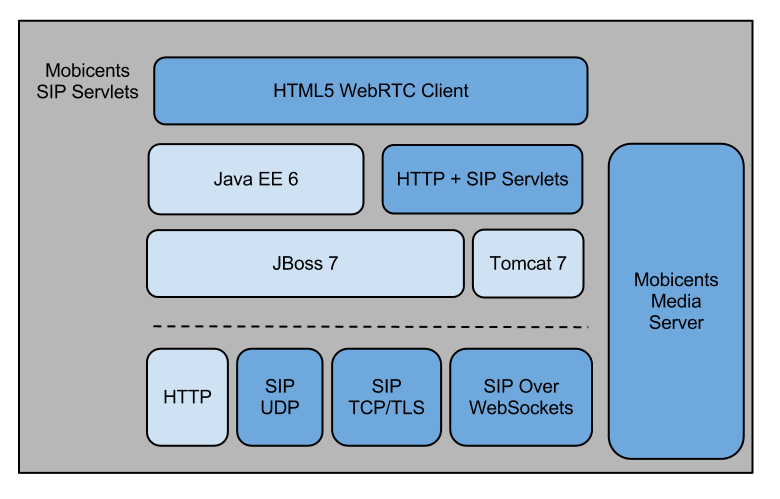
\includegraphics[width=0.60\textwidth,natwidth=610,natheight=642]{figs/mobicents.png}
  	\caption{Mobicents SIP Servlets\cite{code:mobicents}}
  	\label{fig:mobicents}
\end{figure}

\par Mobicents \gls{sip} Servlets delivers a consistent, open platform on which to develop and deploy portable and distributable \gls{sip} and Converged \gls{jee} services.  It is the first open source certified implementation of the \gls{sip} Servlet v1.1 (\gls{jsr} 289 Spec) on top of Tomcat\footnote{Apache Tomcat (or simply Tomcat, formerly also Jakarta Tomcat) is an open source web server and servlet container developed by the Apache Software Foundation (ASF).\cite{wiki:tomcat}} and JBoss\footnote{WildFly, formerly known as JBoss AS, or simply JBoss, is an application server authored by JBoss, now developed by Red Hat. WildFly is written in Java, and implements the Java Platform, Enterprise Edition (Java EE) specification. It runs on multiple platforms.\cite{wiki:jboss}} containers and strive to feature best performances, security, foster innovation and develop interoperability standards between \gls{sip} Servlets and \gls{jslee} so that applications may exploit the strengths of both. The \gls{jain}\footnote{Java APIs for Integrated Networks (JAIN) is an activity within the Java Community Process, developing APIs for the creation of telephony (voice and data) services.\cite{wiki:jain}}-\gls{sip} Reference implementation is leveraged as the \gls{sip} stack and Mobicents \gls{jain} \gls{slee}\footnote{An accelerated development and deployment environment of new IP Multimedia Subsystem (IMS) services for convergent fixed- mobile network environments.\cite{website:slee}} is used as the \gls{slee} implementation.

\par The architecture of the Mobicents \gls{sip} Servlets is shown in Figure \ref{fig:mobicents}. As it described, Mobicents \gls{sip} Servlets provide multiple transport protocol include \gls{http}, \gls{udp}, \gls{tcp} and WebSocket. These transport protocols are fit the prototype requirements, but on the application layer, it has two application server need to be host, one is JBoss and the other is Tomcat 7, JBoss is support for all the \gls{sip} stack transport and Tomcat 7 is support for \gls{http} requests. JBoss is the gateway to communicate with \gls{sip} network and Tomcat host the application server to communicate with media server to handle the real-time multimedia stream.

\par It is quite nice system architecture to work with, but it need powerful server machine to host two web application server on it. Considering Node.js solution, it is not easy to maintain the system since developer need to configure on two different web application server to handle different protocol transportation and client and server are implemented in different programming languages.

\par After implemented one test application by Mobicents \gls{sip} Servlets framework, it is hard for developer to program the lower level source codes, for example \gls{sip} message headers field modification and WebSocket transport template. The test application successes to set up conversation session between \gls{webrtc} browser client and \gls{sip} client. But when the media stream exchange on XMS server(media server), there is only one way audio(from browser to phone) in the conversation. Because the \gls{sip} transport layer is encapsulated in the Mobicents \gls{sip} Servlets framework, it is hard to modify it to do more test if the bug is in the transport layer of the framework. The source code of this test application is owned by Gintel AS.

\par As a conclusion, the prototype system will use Node.js as server side back-end to communicate with AngularJs client application on Socket.IO protocol.